\chapter{Asking Miami Millionaires How They Got Rich}

This chapter follows a School of Hard Knocks interview, curated by LazyingArt LLC, and it is best read as a lecture in operational mathematics rather than symbolic mathematics. We are not given a single formula for wealth. Instead, we are led through a sequence of local rules: save first, scale in stages, test for traction before investing, learn by failing faster, recruit through leadership and product strength, and refuse the distortions created by comparison. The transcript is informal, but its order is careful enough that we can write it as a chain of definitions, inequalities, and causal dependencies.

\section{Miami as a Sampling Device for Wealth Paths}

We begin with a repeated question posed to different people in rapid succession: what would one tell a younger self starting from zero? That repetition is the lecture's opening device. It turns Miami into a sampling apparatus. Social media marketing, commercial real estate, professional sport, and competitive intelligence appear side by side, and the effect is immediate: wealth is not confined to one privileged domain.

The lecture does not slow down at once. It first lets us hear compressed imperatives: fail faster, find mentors, model the right behaviors. It then overlays those imperatives with a catalogue of industries. Only after that breadth is established does the interviewer say, in effect, \emph{we have landed in Miami to ask how millionaires became wealthy}. That explicit framing matters. The lecture is announcing that what follows will not be one biography, but a field survey whose fragments must later be assembled into structure.

The opening therefore fixes two baseline facts. First, starting from zero is the common initial condition. Second, the diversity of careers does not eliminate the possibility of common mechanisms. On the contrary, it is what makes those mechanisms worth isolating.

\section{Savings Discipline and the First Structure of Scale}

The first extended framework comes from a speaker who reports a four-million-dollar year, places himself in business development and sales, and then gives advice that is mathematically modest but structurally important: place a fixed share of income in an index fund and hold that rule constant. In notation,
\begin{equation}
I_{\mathrm{idx}} = 0.10\,Y,
\end{equation}
where $Y$ is income and $I_{\mathrm{idx}}$ is the protected index allocation.

The force of the rule is not that it explains all investing. It does not. The point is that one part of the portfolio is walled off from improvisation. The lecture presents this as a floor: before we speculate, optimize, or signal sophistication, we first create a non-negotiable bucket.

Then the interviewer immediately turns from savings to scale. That juxtaposition is important. The lecture does not let us imagine that private discipline and large-scale growth are separate worlds. The very next question is how a business actually scales, and the speaker answers by dividing growth into distinct tranches:
\begin{equation}
G=\{G_1,G_2,G_3\}.
\end{equation}
Here $G_1$ is the initial stage of blood, sweat, and tears; $G_2$ and $G_3$ are later stages whose demands are different from the first and different from each other.

That is the first real abstraction of the chapter. Growth is not one smooth line. The second hundred million is not produced the way the third is. The lecture's warning is that many people misestimate these tranches by assuming that the next stage is simply more of the same. It is not. Each stage asks for a new source of leverage, a new structure, or a new set of people.

\subsection{Question \& Answer}

The lecture then raises a local obstacle that should remain explicit on the page: how do we get from a seven-figure business to an eight-figure business?

\paragraph{The question.}
How do we tell whether an early success is the beginning of a real growth path rather than a lucky first win?

\paragraph{The answer.}
The lecture answers in a short chain of tests. We first classify the origin of the initial success. It may have come from luck. It may have come from friends and family. It may have come from a good idea that simply does not scale. Only after that diagnosis do we ask the larger question:
\begin{equation}
\text{8-figure scale} \Rightarrow M_{\mathrm{addr}} \text{ is sufficiently large},
\end{equation}
where $M_{\mathrm{addr}}$ is the effective addressable market, the safest formal gloss for what the speaker calls the ``green field.''

The reasoning proceeds step by step.
\begin{enumerate}
\item Do not take the first win as self-validating.
\item Ask whether the market is large enough for the next level.
\item If the market is real, ask what the right path into that market actually is.
\item Bring in people who know how to measure that path rather than trying to solve it alone.
\end{enumerate}

The lecture's emphasis on experts is not ceremonial. It is part of the mathematics of scale. A wrong diagnosis at seven figures is expensive precisely because the next stage magnifies mistakes.

\section{Interlude, Competitive Intelligence, and Traction}

At this point the lecture deliberately loosens its grip. There is crowd noise, repeated thanks, jokes, skepticism, and bystander commentary. That interlude should not be erased in the notes. It is the lecture's pacing reset. The street comes back in before the next concept is introduced.

The next concept arrives through a speaker who calls himself a spymaster. The term is playful, but the definition is sober.

\begin{definition}
\emph{Competitive intelligence} is the disciplined monitoring of a company's external environment in a threat-analysis style: one watches what is happening outside the firm, much as a government watches external and internal threats.
\end{definition}

This matters because it changes the order of operations. We do not begin by allocating capital. We begin by reading the environment. That is why the same speaker's financial advice is to pay oneself first, push resources toward retirement, and then invest only after the field has been examined.

The lecture's investment filter can be written schematically as
\begin{equation}
\text{observation} \Rightarrow \text{traction test} \Rightarrow \text{investment}.
\end{equation}

\begin{definition}
\emph{Traction} is observable evidence that demand is real and that the company is not merely a temporary or ``fly-by-night'' construction.
\end{definition}

The order is crucial. The lecture is not saying merely ``invest in good things.'' It is saying that intelligence comes before allocation. We first ask where there is traction; only then do we move money.

The same speaker then broadens the register and gives the lecture one of its cleanest philosophical pivots. ``You only live once'' is recast into a stronger asymmetry: one dies once, but one lives every day. This is not merely a slogan. It keeps the section from becoming a dry manual of retirement planning. The lecture wants both sides at once: long-horizon discipline and daily seriousness.

\section{Miami, Failure, and the Cost of Significance}

The penthouse interview is a genuine new act. The hosts announce that they have met a successful entrepreneur in Miami, that they are going up to his apartment, and that they want to hear how he thinks. This scene change is not decorative. It marks a shift from quick street rules to a more developed theory of wealth-building.

The first question is why move to Miami. The answer is not about weather or status. It is about atmosphere. Miami is described as a city that does not shame intense work, that normalizes exposure to larger fortunes, and that keeps the many levels of the game visible. In that setting, ambition is not an internal monologue but something reinforced by the environment itself. The speaker's phrase that transformation is ``a mountain with no top'' is not mathematical, but it is structural. It says that exposure changes the scale of the climb one considers normal.

The next move is more technical. Asked what advice he would give his younger self, the speaker says to fail faster and not assign so much significance to each small failure. The lecture's argument is that failure becomes toxic only when it is over-interpreted.

We may summarize the logic as
\begin{align}
\text{smaller emotional penalty} &\Rightarrow \text{faster iteration},\\
\text{faster iteration} &\Rightarrow \text{more learning per unit time},\\
\text{more learning per unit time} &\Rightarrow \text{greater compounded adaptation}.
\end{align}
This is not a visible board derivation from the lecture. It is a cautious transcript-based reconstruction of the mechanism actually described.

\subsection{Question \& Answer}

The lecture then asks a direct explanatory question: why do some ecosystems produce many more billion-dollar startups?

\paragraph{The question.}
Why, in the speaker's telling, does a place such as Israel seem to generate so much entrepreneurial scale?

\paragraph{The answer.}
The transcript gives a mechanism rather than a dataset. The claim is that some environments teach people to fail forward intelligently, to learn from mistakes faster, and to remove false significance from each setback. The argument is sequential:
\begin{enumerate}
\item strip failure of theatrical meaning;
\item shorten the interval between attempt and correction;
\item make the next attempt quickly;
\item let those faster cycles compound over time.
\end{enumerate}

The notes should keep the claim cautious. The transcript is rhetorically strong and statistically loose. But its mechanism is clear enough: ecosystems outperform when they make iteration cheap in psychic terms and therefore frequent in practical terms.

This is also where the lecture names Ryan Breslow as a studied example. The function of that example is not celebrity. It is to bridge from ecosystem-level thinking to firm-level mechanics. The next section makes that bridge explicit.

\section{The Dependency Chain of Scale}

Once Ryan Breslow is introduced, the lecture compresses its main thesis into two words: fundraising and recruiting. But it does not leave those words standing alone. As the speaker continues, they unfold into a hierarchy.

\begin{remark}
Since no validated board figure survives for this lecture, the chain below is a cautious transcript-based schematic rather than a transcription of visible notation.
\end{remark}

The transcript supports the following relations:
\begin{align}
Q &\Rightarrow V \Rightarrow L,\\
L &\Rightarrow R,\\
F &\Rightarrow K \Rightarrow \text{scale},\\
Q &\Rightarrow C \Rightarrow T.
\end{align}
Here $Q$ is product quality, $V$ visionary clarity, $L$ leadership, $R$ recruiting capacity, $F$ fundraising, $K$ deployable cash, $C$ compensation capacity, and $T$ top-tier talent.

The lecture's point is not that these arrows form a perfectly linear theorem. It is that scale depends on stacked conditions. Cash is needed to scale. Cash at speed often comes through fundraising. Recruiting depends on leadership. Leadership depends on vision. Vision depends on a genuinely strong product. Talent depends not just on the desire to hire, but on the ability to compensate at a level that serious people will accept.

We may draw the chain as follows.

\begin{figure}
\centering
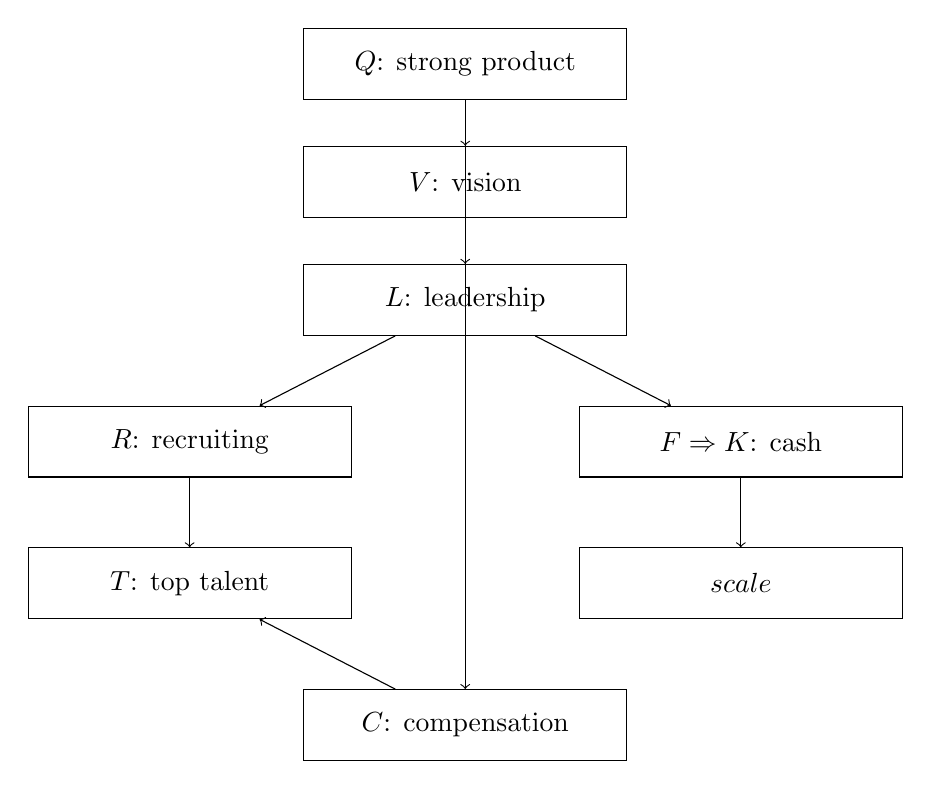
\begin{tikzpicture}
\node[draw, rectangle, minimum width=4.1cm, minimum height=0.9cm] (q) at (0,0) {$Q$: strong product};
\node[draw, rectangle, minimum width=4.1cm, minimum height=0.9cm] (v) at (0,-1.5) {$V$: vision};
\node[draw, rectangle, minimum width=4.1cm, minimum height=0.9cm] (l) at (0,-3.0) {$L$: leadership};

\node[draw, rectangle, minimum width=4.1cm, minimum height=0.9cm] (r) at (-3.5,-4.8) {$R$: recruiting};
\node[draw, rectangle, minimum width=4.1cm, minimum height=0.9cm] (f) at (3.5,-4.8) {$F \Rightarrow K$: cash};

\node[draw, rectangle, minimum width=4.1cm, minimum height=0.9cm] (t) at (-3.5,-6.6) {$T$: top talent};
\node[draw, rectangle, minimum width=4.1cm, minimum height=0.9cm] (s) at (3.5,-6.6) {$\text{scale}$};

\node[draw, rectangle, minimum width=4.1cm, minimum height=0.9cm] (c) at (0,-8.4) {$C$: compensation};

\draw[->] (q) -- (v);
\draw[->] (v) -- (l);
\draw[->] (l) -- (r);
\draw[->] (r) -- (t);
\draw[->] (l) -- (f);
\draw[->] (f) -- (s);
\draw[->] (q) -- (c);
\draw[->] (c) -- (t);
\end{tikzpicture}
\end{figure}

The lecture then introduces an industry contrast. In e-commerce, one sometimes imagines one product, one platform, one ad engine, and then extension from there. In finance, private equity, and technology, the stress falls more heavily on top-tier talent. The notes should preserve the contrast exactly at this moment, because it explains why the chain branches. In some sectors product-market fit dominates the early picture; in others the decisive constraint is the people one can afford to bring in.

\section{Brickell: Institutional Work, Relationships, and Product Economics}

After the penthouse segment the lecture returns to the street. The hosts announce that they have made it to Brickell and will ask more multimillionaires how they became financially free. This reset matters, because the lecture now replays its themes in shorter modules.

The first Brickell speaker is a software engineer who works for himself and builds apps for Penn State University, Lockheed Martin, and the state of Texas. He reports a two-million-dollar year. The point is not simply that software can pay. The point is that technical work becomes economically powerful when it becomes legible to institutions.

The next rule is that relationships are everything. But again the lecture refuses to leave the claim vague. One must come to the table with something to offer. We should therefore read the advice not as networking sentiment but as a rule about exchange: relationship capital is created when one arrives with value already in hand.

The same speaker then gives a second numerical rule:
\begin{equation}
s=0.70,\qquad c=0.30,\qquad s+c=1,
\end{equation}
where $s$ is the saving share and $c$ is the operating or spending share. He pairs this with a recommendation to leverage credit so as to preserve cash.

\paragraph{Worked Example.}
The lecture itself supplies a two-million-dollar annual income in this segment. Using that number only as an illustrative arithmetic input, the 70/30 rule gives
\begin{align}
sY &= 0.70Y = \$1{,}400{,}000,\\
cY &= 0.30Y = \$600{,}000.
\end{align}
By comparison, the earlier rule isolates
\begin{equation}
I_{\mathrm{idx}}=0.10Y=\$200{,}000.
\end{equation}
The notes should state plainly that these are different speaker-specific heuristics, not one unified doctrine. Their common content lies elsewhere: income must be partitioned by rule before mood and status consume it.

The next speaker recounts a path from social media marketing to owned e-commerce brands. That transition is a major one. The speaker realizes that agency work can still leave one under the command of clients, and he moves from servicing brands to owning them. That is the lecture's shift from fee income to brand equity.

Brand is then described through a vivid response structure. A sufficiently strong brand changes the customer's question. The customer no longer asks why one should jump. The customer asks only how high. Apple functions as the canonical example, not because the lecture gives a clean financial decomposition of Apple, but because it wants to make the mechanism clear: a strong brand lowers the friction of demand across adjacent products.

That leads directly to the sharpest e-commerce rule in the lecture:
\begin{equation}
Q \succ Mkt \succ Sal,
\end{equation}
where $Q$ is product quality, $Mkt$ is marketing, and $Sal$ is sales. The speaker immediately adds two directional consequences:
\begin{align}
Q \uparrow &\Rightarrow \text{need}(Mkt)\downarrow,\\
Mkt \uparrow &\Rightarrow \text{need}(Sal)\downarrow.
\end{align}
The point is not that marketing or sales vanish. The point is that a strong product changes the burden carried by the later layers.

\section{Place, Pressure, Real Estate, and the Comparison Trap}

The lecture now widens again. The same Brickell stretch asks what Miami has done to one's mindset. The answer is that the city makes one want to level up, hustle harder, and treat ordinary standards as too small. Another speaker, a professional soccer player, answers success in a different key: he performs best under pressure and under responsibility. The lecture is still on the same theme. Environment and pressure are not distractions from performance. They are part of the mechanism by which performance is intensified.

The motif of modeled behavior then returns explicitly. Another interviewee says: ask a lot of questions, find mentors, and model what they do. The lecture thereby reconnects to its opening instruction. The city changes the scale of the game, but imitation remains one of the basic technologies of entry.

The commercial real-estate segment makes these abstractions concrete. A building is chosen because it lies between I-95 and the Florida Turnpike, so that the entire property set remains within workable reach:
\begin{equation}
\forall i,\qquad t_i \le 3\,\mathrm{h}.
\end{equation}
This is not geometry for its own sake. It is logistics turned into economic advantage.

The Celsius story then shows why place matters beyond convenience. Office ownership is not merely rent extraction. It is adjacency to people, firms, and weak signals that may later become large opportunities:
\begin{equation}
O_{\mathrm{office}} \Rightarrow \text{tenant contact} \Rightarrow \text{acquisition opportunity} \Rightarrow \text{equity upside}.
\end{equation}
The speaker's point is that a building can be a node in a network of encounters. Ownership changes what one gets to see, and what one gets to see changes what one can buy.

The lecture closes with a warning that is psychological and financial at once. Do not count other people's money. Much of what appears on the social surface is fake or exaggerated; comparison creates insecurity, and insecurity produces foolish spending. In compact form,
\begin{equation}
\text{comparison} \Rightarrow \text{insecurity} \Rightarrow \text{distorted spending}.
\end{equation}
The final instruction is therefore not simply moral. It is allocative. Worry about yourself, move at your own pace, and refuse to spend in obedience to another person's performance.

\section{Summary}

The lecture begins with many industries and ends with a small number of repeatable mechanisms. Save first. Treat growth as staged. Do not mistake an early win for a scalable market. Read the environment before investing. Let failure become information rather than identity. Build product before amplifying it. Remember that talent depends on compensation, compensation depends on economic strength, and location changes the opportunity set one can even perceive.

What makes the transcript useful is precisely that it does not pretend to be one polished theorem of wealth. It unfolds as a guided accumulation of rules, examples, and local explanations. The chapter's job is therefore not to force a false unity, but to preserve the lecture's sequence while extracting its durable mathematics: partitions of income, staged growth, priority orderings, dependency chains, logistical constraints, and behavioral feedback loops. Those are the objects that remain when the street noise falls away.